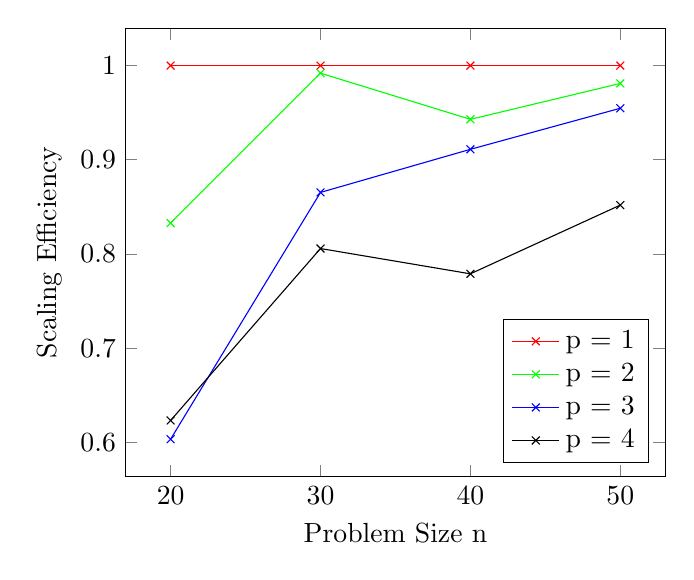
\begin{tikzpicture}
\begin{axis} [xlabel=Problem Size n, ylabel=Scaling Efficiency, xtick = {1, 2, 3, 4}, xticklabels = {20,30,40,50}, ytick = {0.6, 0.7, 0.8, 0.9, 1.0}, legend pos = south east]
\addplot[color=red, mark=x] coordinates {
(1, 1.0000000000000000)
(2, 1.0000000000000000)
(3, 1.0000000000000000)
(4, 1.0000000000000000)
};
\addlegendentry{p = 1}\addplot[color=green, mark=x] coordinates {
(1, 0.8327444749790944)
(2, 0.9919300936424615)
(3, 0.9429213373822428)
(4, 0.9810451159330554)
};
\addlegendentry{p = 2}\addplot[color=blue, mark=x] coordinates {
(1, 0.6033018605045571)
(2, 0.8653397310326268)
(3, 0.9110892397308801)
(4, 0.9546862471285500)
};
\addlegendentry{p = 3}\addplot[color=black, mark=x] coordinates {
(1, 0.6232019592686404)
(2, 0.8057410122532163)
(3, 0.7788889933187060)
(4, 0.8518654908062756)
};
\addlegendentry{p = 4}\end{axis}
\end{tikzpicture}
